\section{Appendix: Details on local methods}

\subsection{AD-enabled design optimization}

To develop a general-purpose, efficient, and robust design optimization framework for autonomous systems, we must address three main challenges. First, how can we ensure that the system is \textit{flexible}, not requiring large amounts of work to specialize the framework to particular application domains. Second, how can we incorporate \textit{robustness} into the design optimization process, to minimize the sensitivity of the optimized design to variation in the exogenous parameters. Finally, how can we achieve both of these goals \textit{efficiently}, making use of gradients wherever possible to accelerate the search for high-performing designs.

\paragraph{Flexibility} Most robots are composed of many interacting subsystems, and different subsystems are typically modeled using different levels of abstraction. Although some tools may aid in designing certain subsystems (e.g. Simulink for controllers, SolidWorks for hardware), these tools cover only a small part of the overall robotics design problem, which includes sensing, actuation, perception, navigation, control, and decision-making subsystems. Since few robotic systems are exactly alike, an effective design tool must allow the user to select an appropriate level of abstraction for the problem at hand.

When it comes to managing complexity in a general-purpose design framework, programming languages are a natural tool. They allow users (i.e. programmers) to define precisely which abstractions are appropriate for any given application (e.g. by defining appropriate class hierarchies and function interfaces) without sacrificing generality. To take advantage of this expressivity, we can view engineering designs as programs that define the behavior of the system given suitable choices for design structure and parameters. We can then use automatic differentiation to derive gradients connecting these parameters to the system's behavior and optimize accordingly. This view is inspired by recent work in 3D design optimization~\cite{cascaval2021differentiable}, aircraft design~\cite{sharpe_thesis}, and machine learning~\cite{paszkePyTorchImperativeStyle2019,jax2018github}.

\paragraph{Robustness} Robots operate in dynamic environments that cannot be fully specified \textit{a priori}, and nonlinear interactions between the robot and its environment can make this uncertainty difficult to quantify. Nevertheless, we must account for this uncertainty during the design process and ensure that our designs perform robustly.

Due to this uncertainty, simply minimizing the expected value of the cost $\expectation_{y \sim \cY} \big[ J\pn{S\pn{x, y}} \big]$ can lead to myopic behavior where exceptional performance for some values of $y$ compensates for poor performance on other values; this is related to the phenomenon of ``reward hacking'' in reinforcement learning~\cite{amodei2016_ai_safety}. Ideally, we would like our designs to be robust to variations in exogenous parameters: changing $y$ should not cause the performance to change much. We can include this requirement as a heuristic by penalizing the variance of $J$. Intuitively, this heuristic ``smooths'' the cost function with respect to the exogenous parameters: regions of high variance (containing sharp local minima) are penalized, while regions of low variance are rewarded. This heuristic leads us to the \textit{variance-regularized robust design optimization problem}:
\begin{subequations}\label{app:ch5:eq:design_optimization_nlp_generic}
    \begin{align}
        \min_{x \in \cX} & \quad \expectation_{y \sim \cY} \Big[ J\circ S\pn{x, y} \Big] + \lambda \rm{Var}_{y\sim\cY}\Big[ J\circ S\pn{x, y} \Big] \label{app:ch5:eq:design_optimization_objective_generic}
    \end{align}
\end{subequations}
Practically, we replace the expectation and variance with unbiased estimates over $N$ samples $y_i \sim \cY, i=1,\ldots,N$.
\begin{subequations}\label{app:ch5:eq:design_optimization_nlp}
    \begin{align}
        \min_{x \in \cX} & \quad \frac{1}{N}\sum_{i=1}^{N} \Big[J\circ S\pn{x, y_i}\Big] + \lambda \left[ \frac{\sum_{i=1}^N \pn{J\circ S\pn{x, y_i}}^2}{N-1} - \frac{\pn{\sum_{i=1}^N J\circ S\pn{x, y_i}}^2}{(N-1)N} \right] \label{app:ch5:eq:design_optimization_objective}
    \end{align}
\end{subequations}

\paragraph{Efficiency} Of course, this Monte-Carlo estimate of the variance will require multiple evaluations of $J\circ S$ (where $\circ$ denotes function composition) to evaluate~\eqref{app:ch5:eq:design_optimization_objective}. Since $S$ might itself be expensive to evaluate, approximating the gradients of \eqref{app:ch5:eq:design_optimization_objective} using finite differences or a stochastic gradient estimate will impose a large computational cost ($2nN$ additional evaluations of $J\circ S$ and $c_i$ at each step for finite differences). Instead, we can turn to automatic differentiation (AD) to directly compute these gradients with respect to $x$, which we can use with any off-the-shelf gradient-based optimization engine. The precise choice of optimization algorithm is driven by the constraints and is not central to our framework. If $\cX$ is defined by hyper-rectangle bounds on $x$, then algorithms like L-BFGS-B may be used, but if the constraints are more complex then sequential quadratic programming or interior-point methods may be used.

In this framework, the user need only implement the simulator and cost function for their specific problem using a differentiable programming framework like the JAX library for Python~\cite{jax2018github}, and this implementation can be used automatically for efficient gradient-based optimization. By implementing a library of additional building blocks in this AD paradigm (e.g. estimation algorithms like the EKF), we can provide an AD-based design optimization tool that strikes a productive balance between flexibility and ease of use.

\subsection{Details on multi-agent manipulation case study}

Consider a case study where two mobile robots must collaborate to move a large object. In this setting, two ground robots must collaborate to push a box from its current location to a target pose (as in Fig.~\ref{ch5:fig:mam_hw}). Given the desired box pose and the current location of each robot, a neural network plans a trajectory for each robot, which the robots then track using a feedback controller ($x$ includes both the neural network parameters and the tracking controller gains, with a total of 454 design parameters). The exogenous parameters include the coefficient of friction for each contact pair, the mass of the box, the desired pose of the box, and the initial pose for each robot (a total of 13 exogenous parameters; we vary the desired box pose and initial robot poses to prevent over-fitting during optimization). The cost function is simply the squared error between the desired box pose (including position and orientation) and its true final pose after a \SI{4}{s} simulation. We implement the contact dynamics simulator, trajectory planning neural network, and path tracking controller in Python using JAX.

This case study involves interactions between planning and control subsystems, complicated dynamics, and a high-dimensional design space (>400 design parameters). This example also showcases a different interpretation of the exogenous parameters: instead of representing true sources of randomness, these parameters represent quantities that are simply unknown at design-time. For example, the target position for the box is not random in the same way as sensor noise in the previous example, but since we cannot choose this value at design-time it must be included in $y$. As a result, minimizing the expected cost with respect to variation in $y$ yields a solution that achieves good performance for many different target poses, enabling the user to select one at run-time and be confident that the design will perform well.

To solve this design problem, the neural network parameters are initialized i.i.d. according to a Gaussian distribution, and the tracking controller gains are set to nominal values. We then optimize the parameters using $N = 512$, $\lambda = 0.1$, and L-BFGS-B back-end. This optimization took 45 minutes \SI{32}{s} on a laptop computer with no GPU (\SI{8}{GB} of RAM and a \SI{1.8}{GHz} 8-core CPU). Fig.~\ref{ch5:fig:mam_hw} shows a comparison between the initial and optimized strategies, and Fig.~\ref{ch5:fig:mam_more} in the appendix shows additional examples of the optimized behavior. The target pose is drawn uniformly $[p_x, p_y, x] \in[0, 0.5]^2 \times [-\pi/4, \pi/4]$, and the optimized design achieves a mean squared error of $0.0964$.

We tested the optimized design in hardware, again using the Turtlebot 3 platform. An overhead camera and AprilTag~\cite{olson2011tags} markers were used to obtain the location of the box and each robot. At execution, each robot first moves to a designated starting location near the box, plans a trajectory using the neural network policy, and tracks that trajectory at \SI{100}{Hz} until the box reaches its desired location or a time limit is reached. Results from this hardware experiment are shown in Fig.~\ref{ch5:fig:mam_hw}, and a video is included in the supplementary materials. No parameter tuning or estimation was needed to transfer to hardware.

\begin{figure}[t]
    \centering
    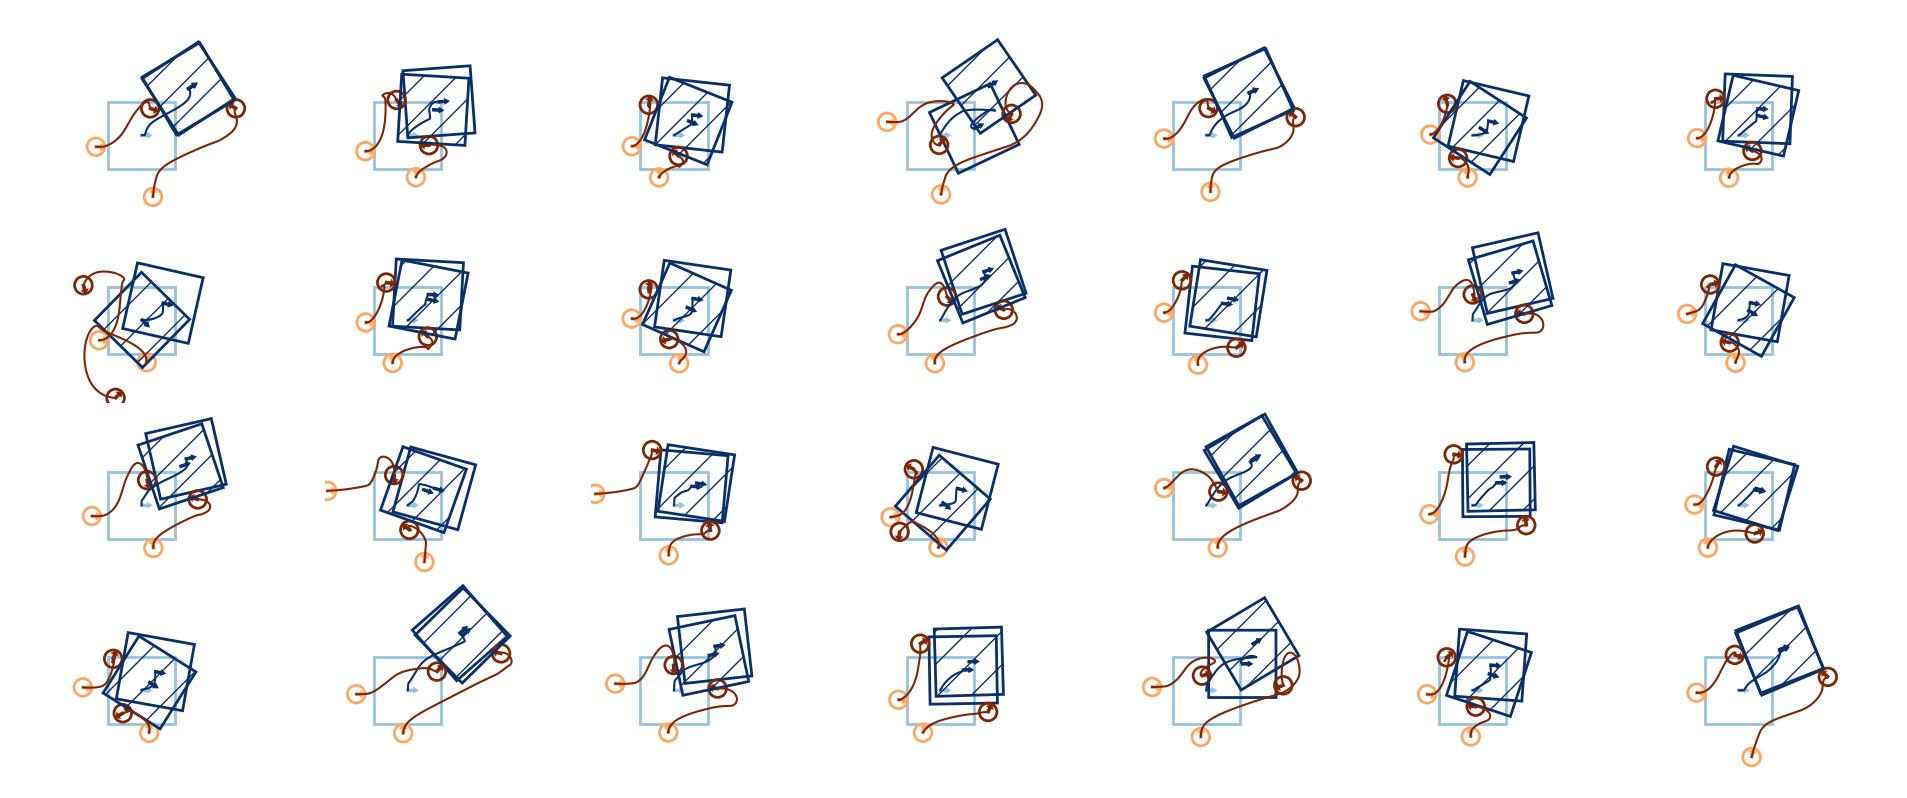
\includegraphics[width=\linewidth]{images/ch5/mam_more.png}
    \caption{Additional examples of optimized multi-agent manipulation behavior in simulation, showing that the optimized strategy reaches the goal in most cases. Each example shows the results of executing the optimized pushing strategy for \SI{4}{s} with a randomly selected set of friction coefficients, random target pose, and random initial robot poses. Light/dark colors indicate initial/final positions, and the striped box indicates the target pose.}
    \label{app:ch5:fig:mam_more}
\end{figure}

To assess the robustness and efficiency of this design optimization method, we must answer a number of questions. For instance, how does automatic differentiation compare with other methods for estimating the gradient (e.g. finite differences)? What benefit does variance regularization in problem~\eqref{ch5:eq:design_optimization_nlp} bring? We answer these questions here using an ablation study where we attempt to isolate the impact of each of these features.

First, why use automatic differentiation? On the one hand, AD allows us to estimate the gradient with only a single evaluation of the objective function, while other methods (such as finite differences, or FD) require multiple evaluations. On the other hand, AD necessarily incurs some overhead at runtime, making each AD function call more expensive than those used in an FD scheme. Additionally, some arguments~\cite{suh2021_bundled_gradients} suggest that exact gradients may be less useful than finite-difference or stochastic approximations when the objective is stiff or discontinuous. We compare AD with a 3-point finite-difference method by re-solving problem~\eqref{ch5:eq:design_optimization_nlp} for both case studies, keeping all parameters constant ($N=512$, $\lambda=0.1$, same random seed) and substituting the gradients obtained using AD for those computed using finite differences. Fig.~\ref{ch5:fig:ablation} shows the results of this comparison. In the sensor placement example, AD achieves a lower expected cost and cost variance, and it runs in 32\% less time. In the collaborative manipulation example, both methods achieve similar expected cost and variance, but the AD version runs nearly 19x faster. These results lead us to conclude that AD enables more effective optimization than finite differences and is an appropriate choice for our framework.

The next question is whether variance regularization brings any benefit to the design optimization problem. To answer this question, we compare the results of re-solving both case studies with variance weight $\lambda = 0.1$ and $\lambda = 0$. These results are shown in Fig.~\ref{ch5:fig:ablation}; surprisingly, in the sensor placement example we see that the variance-regularized problem results in a lower expected cost, contrary to the intuition that regularization requires a trade off with increased expected cost. We expect that this lower expected cost may be a result of the regularization term smoothing the objective with respect to the exogenous parameters. However, these benefits are less pronounced than the benefits from automatic differentiation, and we see more benefit in the sensor-placement example reported in~\cite{dawsonCertifiableRobotDesign2022a} than in the multi-agent manipulation problem.

\begin{figure}[t]
    \centering
    \begin{subfigure}[t]{0.25\linewidth}
        \centering
        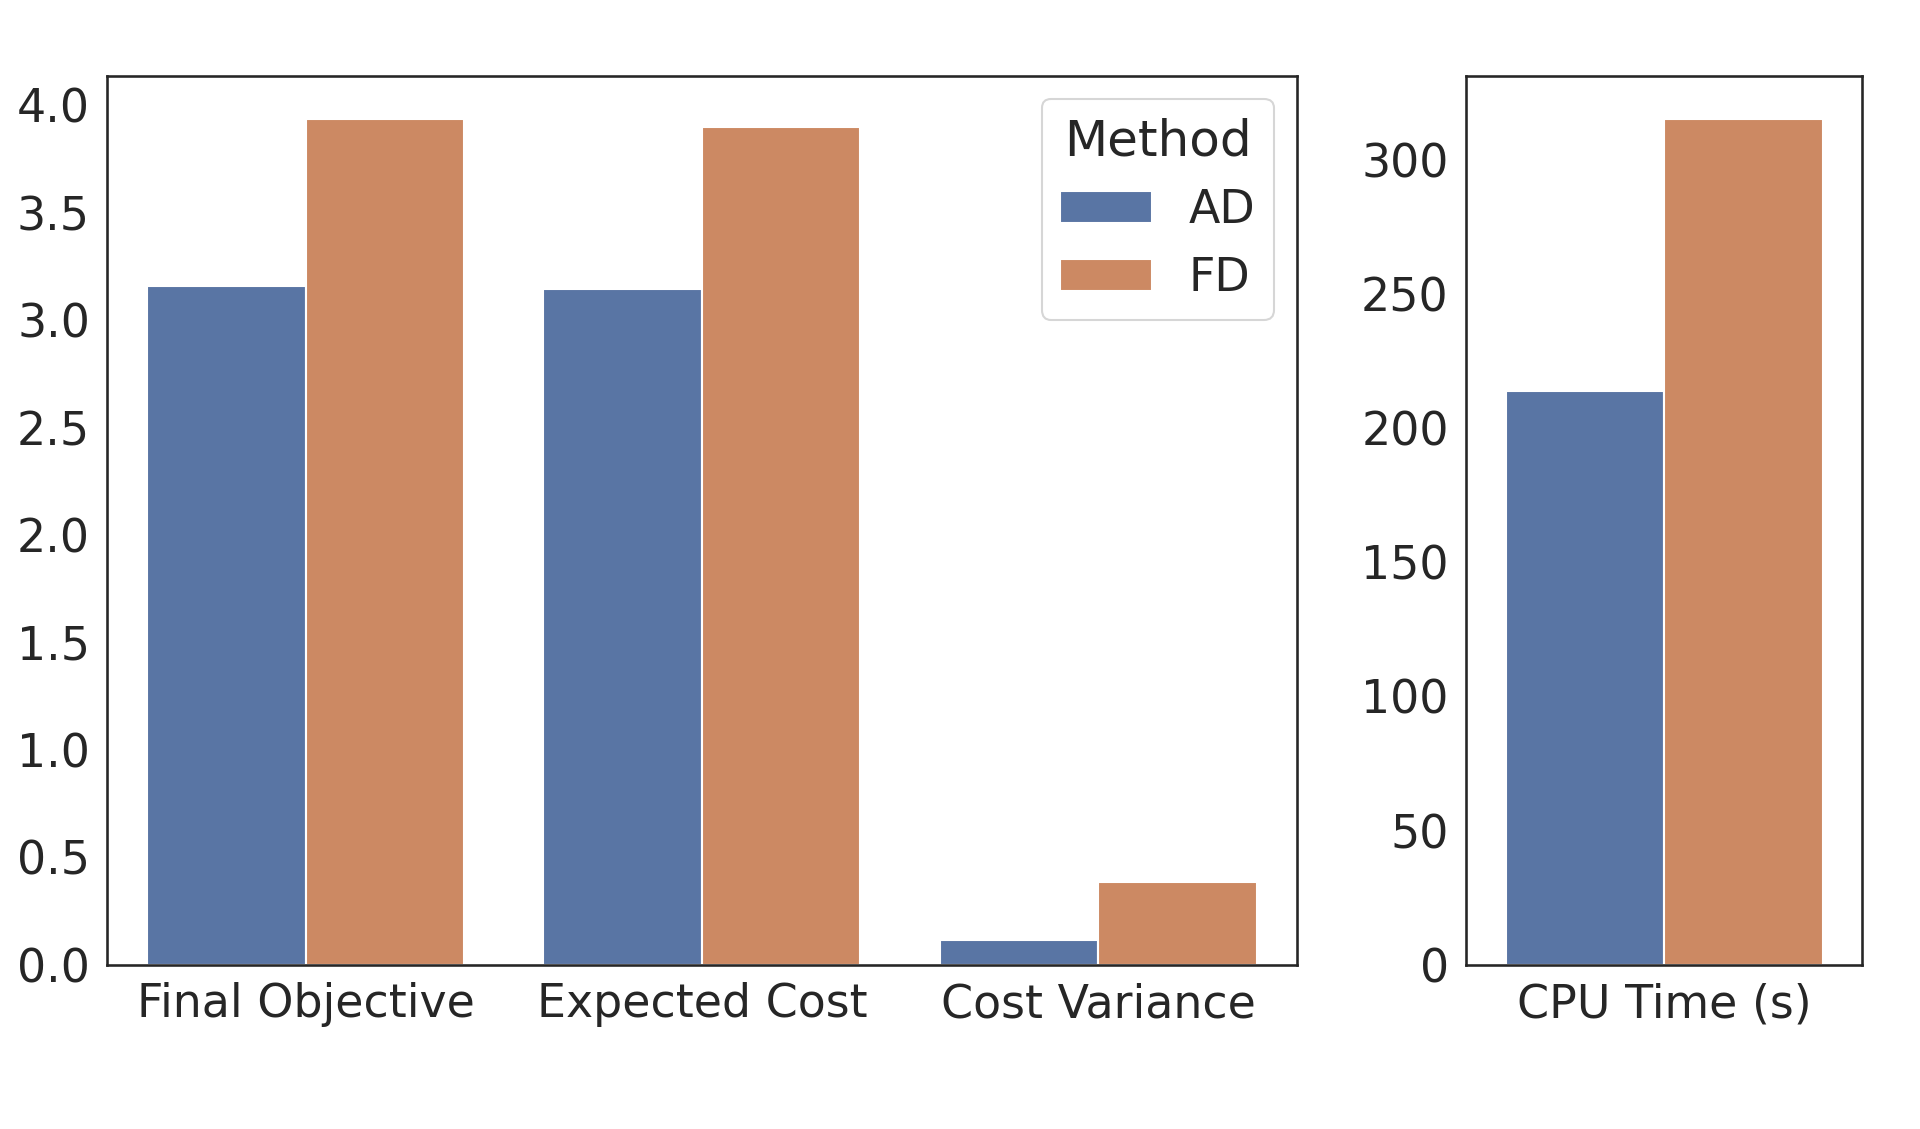
\includegraphics[width=\linewidth]{images/ch5/agv_ad_fd_ablation.png}
        \caption{AD vs. FD; sensor placement}
    \end{subfigure}%
    % \ \\
    % \ \\
    \begin{subfigure}[t]{0.25\linewidth}
        \centering
        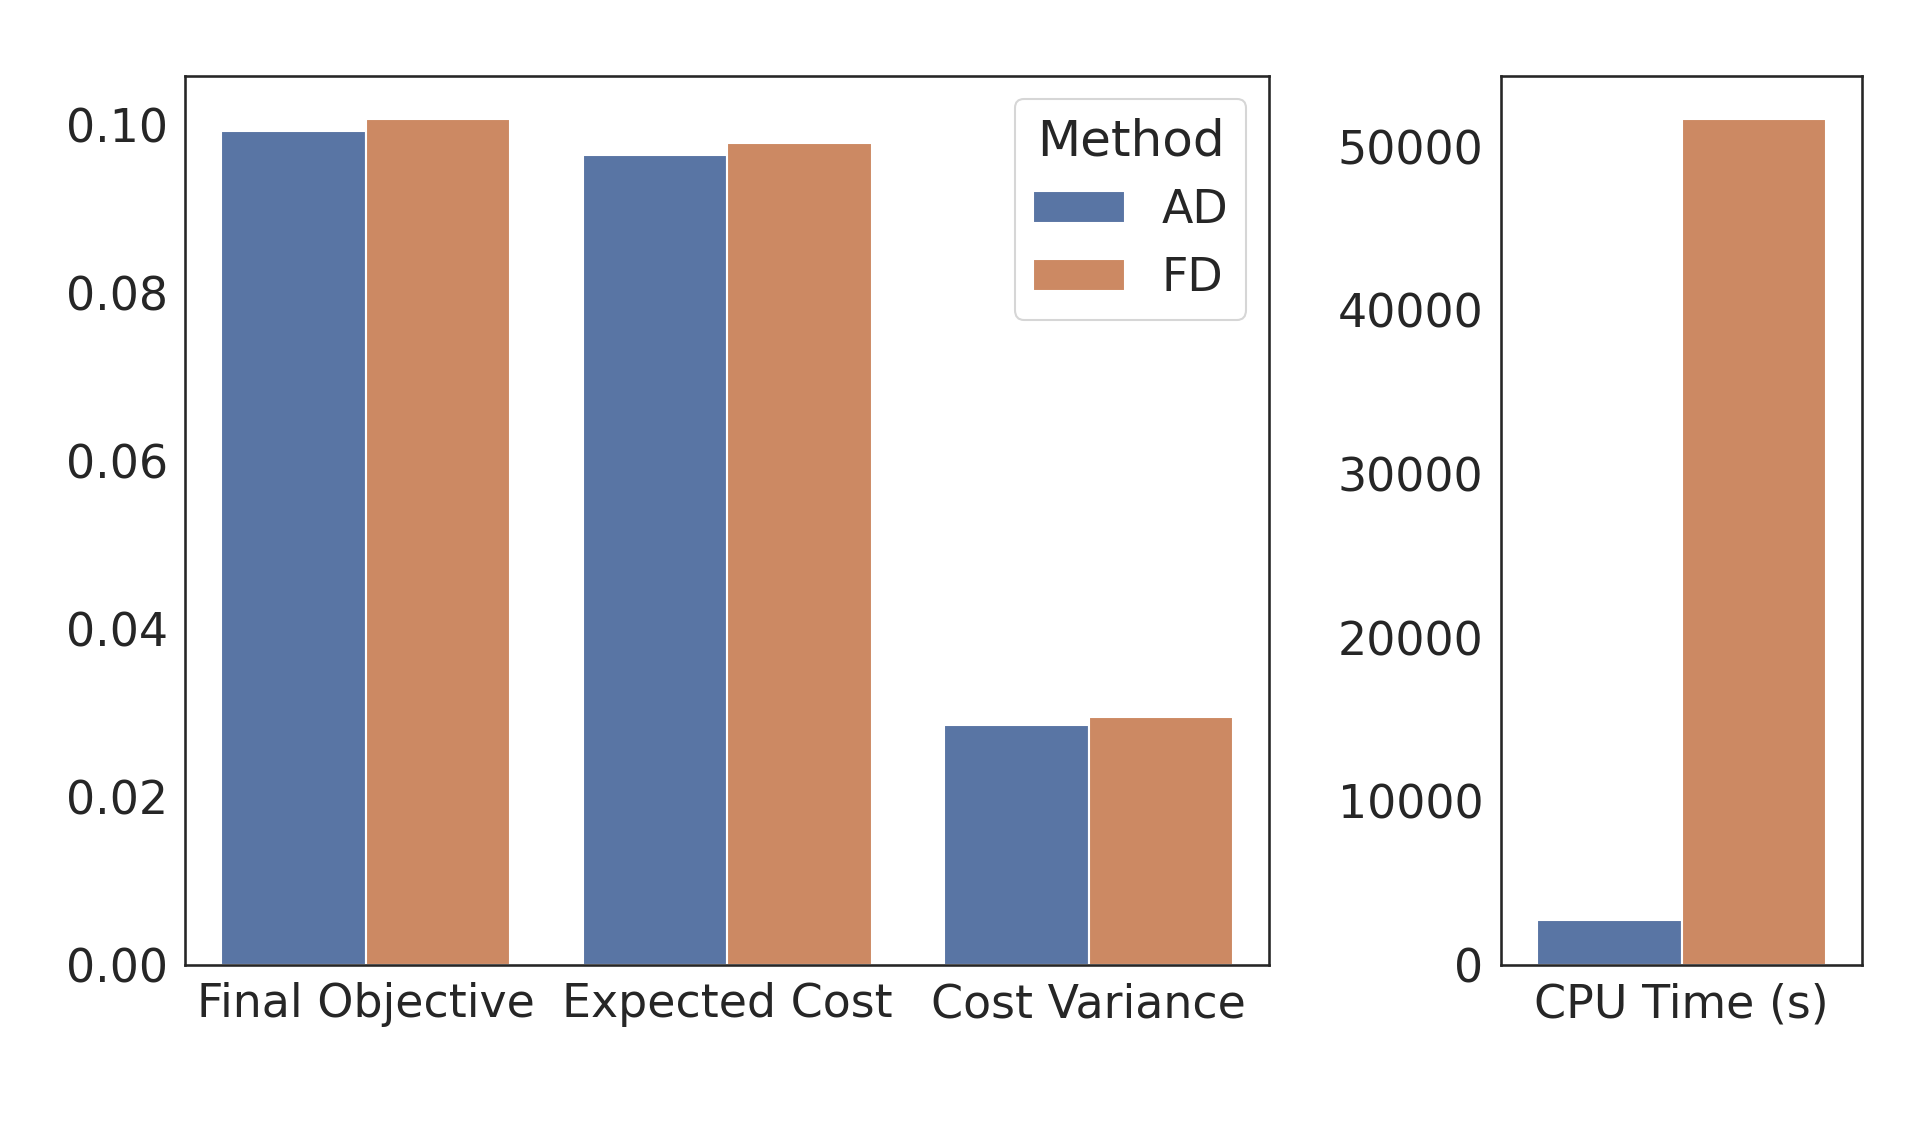
\includegraphics[width=\linewidth]{images/ch5/mam_ablation_ad_fd.png}
        \caption{AD vs. FD; manipulation}
    \end{subfigure}%
    \begin{subfigure}[t]{0.25\linewidth}
        \centering
        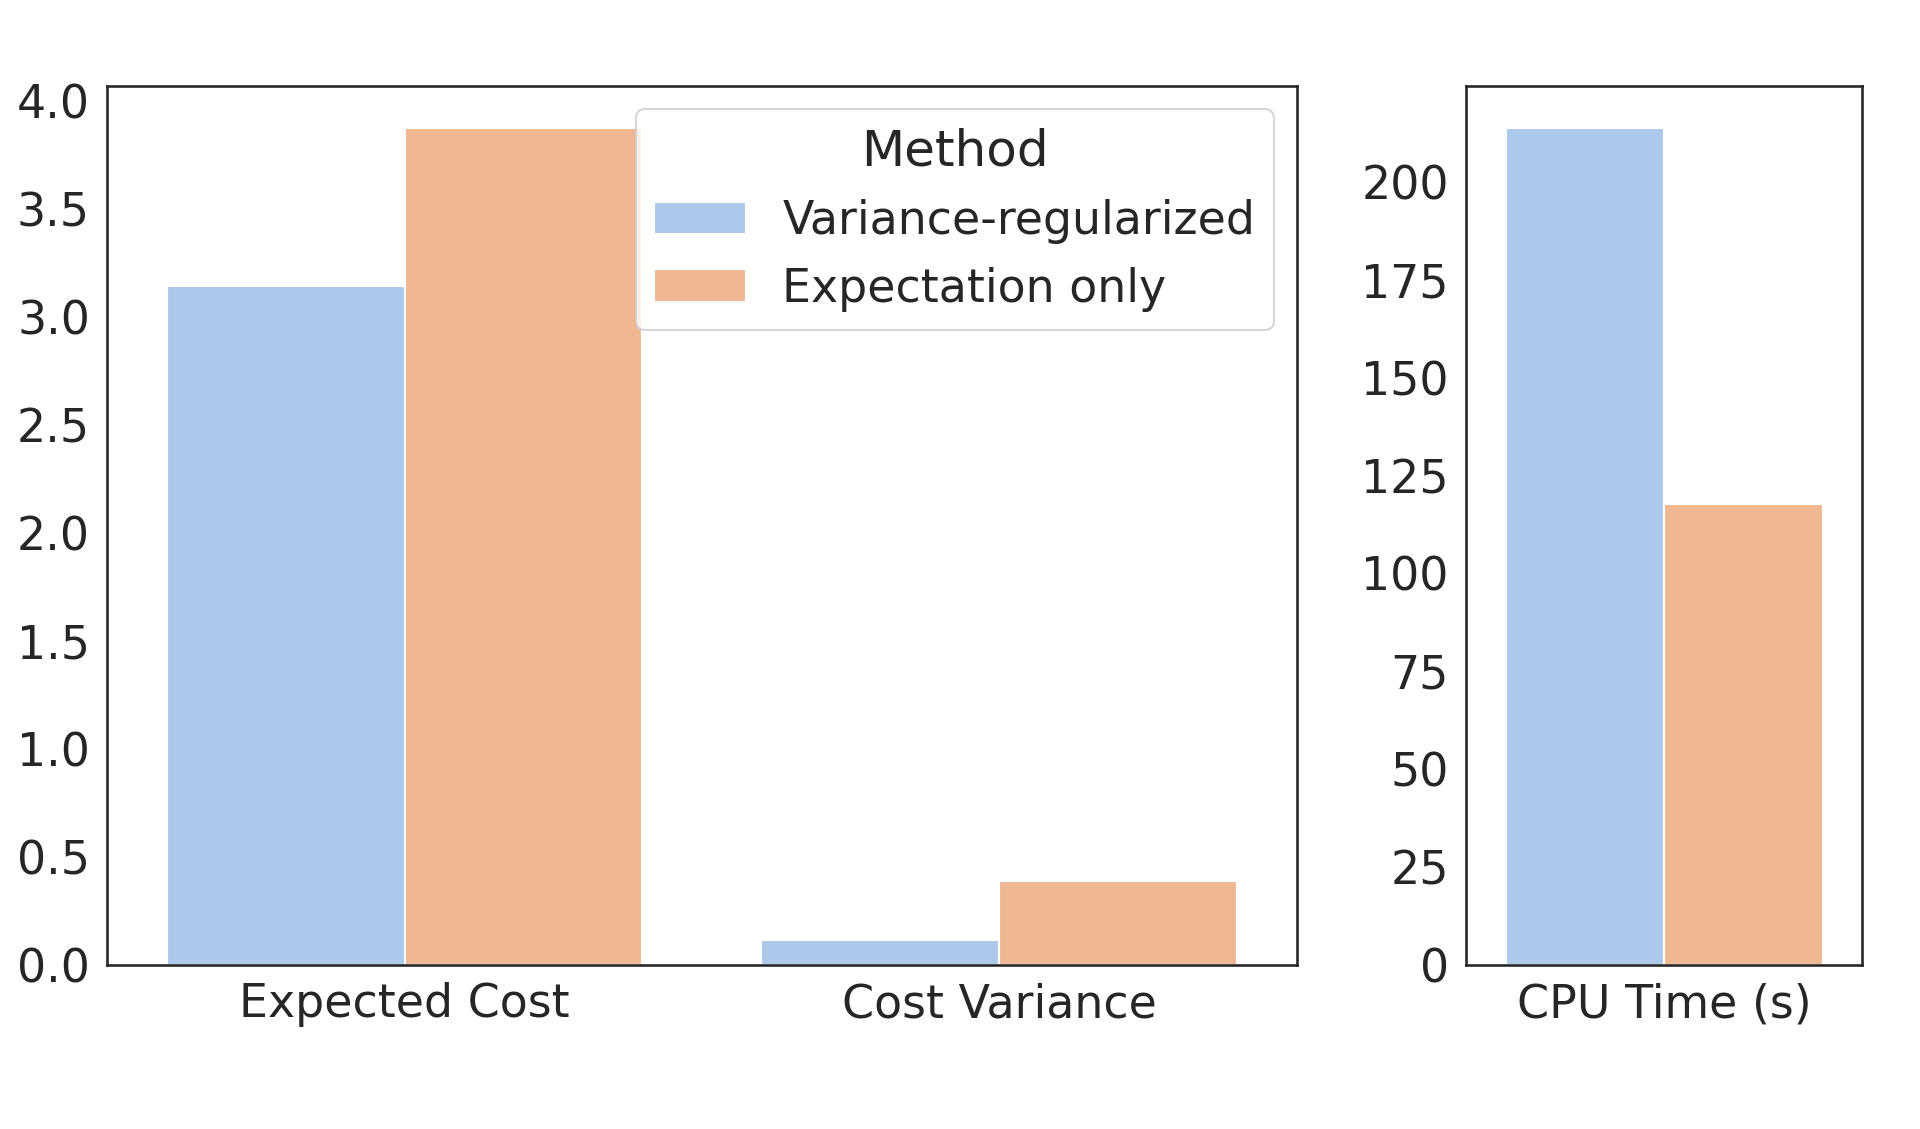
\includegraphics[width=\linewidth]{images/ch5/agv_vr_ablation.png}
        \caption{VR; sensor placement}
    \end{subfigure}%
    % \ \\
    % \ \\
    \begin{subfigure}[t]{0.25\linewidth}
        \centering
        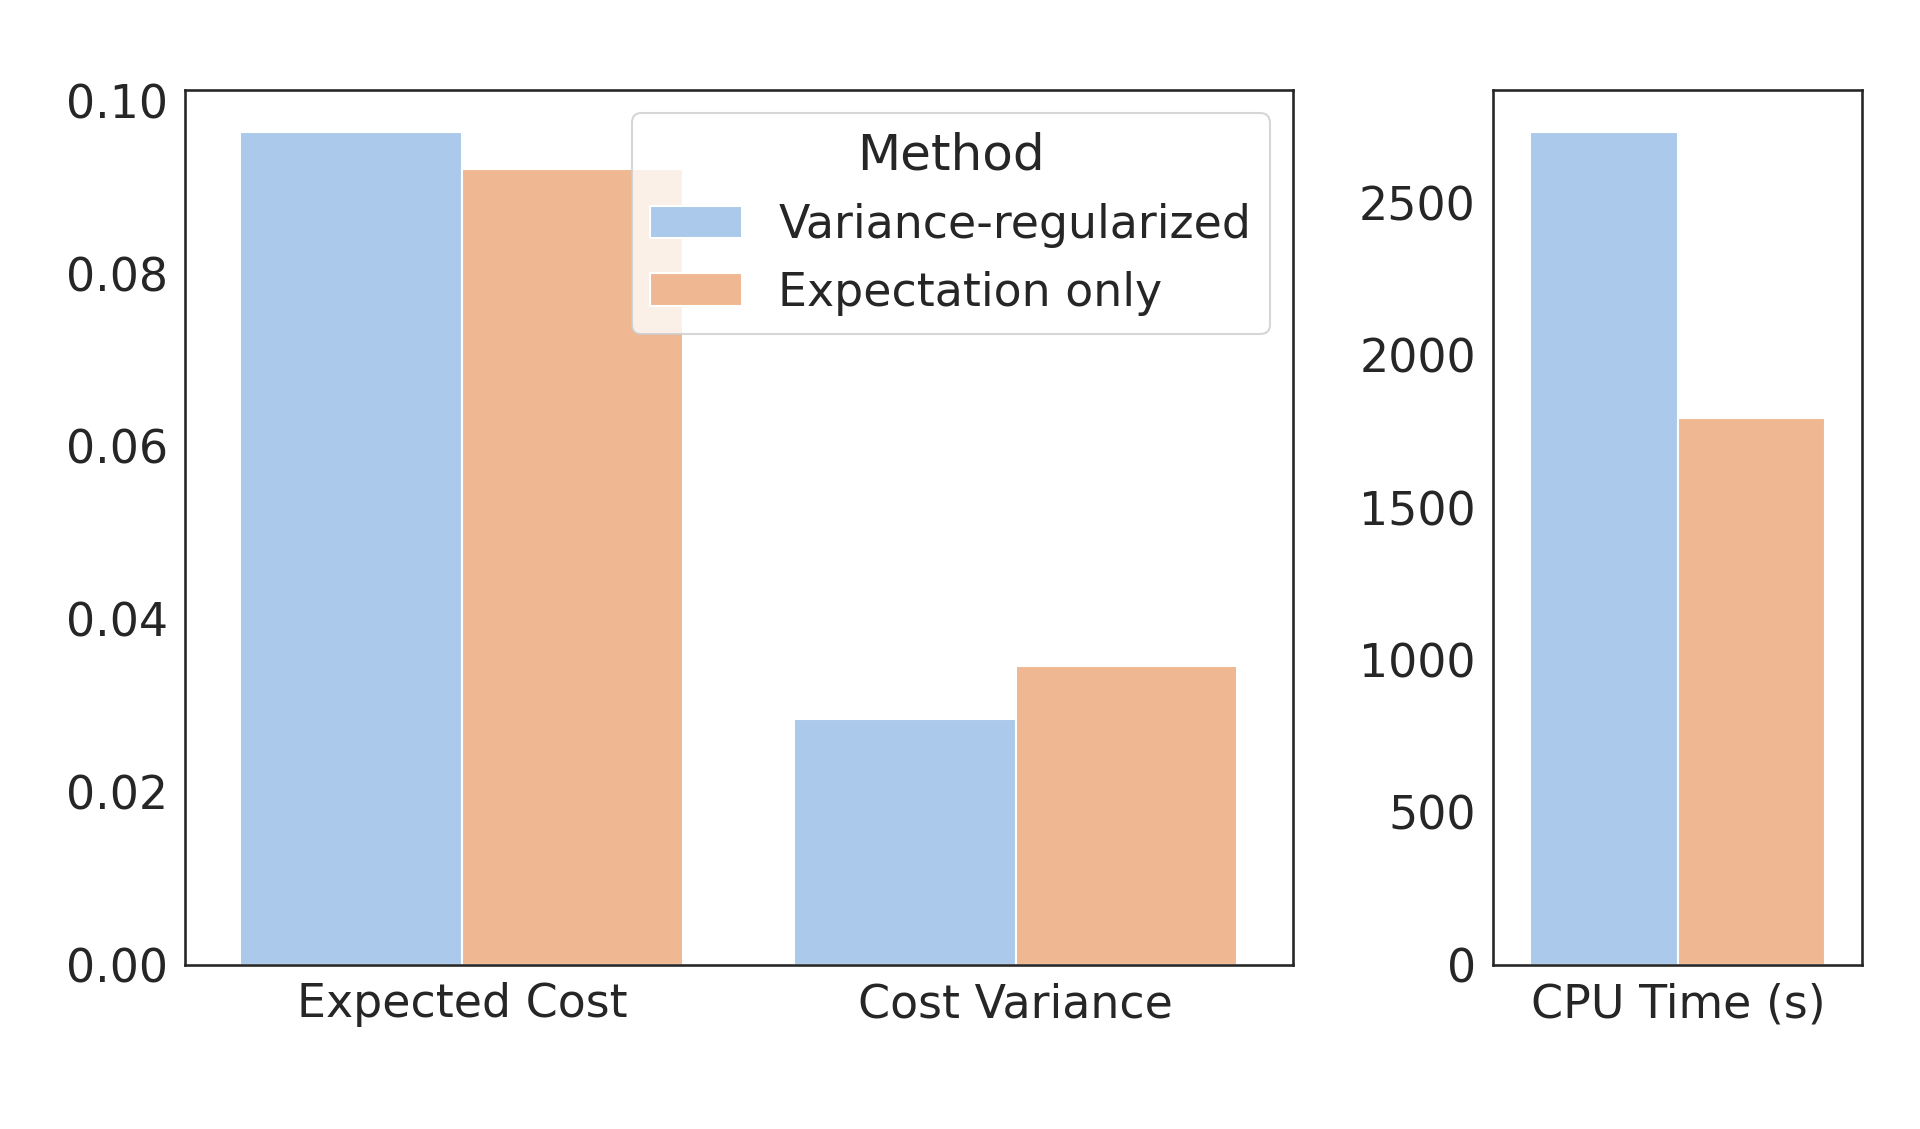
\includegraphics[width=\linewidth]{images/ch5/mam_ablation_vr.png}
        \caption{VR; manipulation}
    \end{subfigure}
    \caption{(a)-(b) Improvement of automatic differentiation (AD) over finite differences (FD) in both case studies. (c)-(d) Effect of variance regularization (VR) in both case studies.}
    \label{app:ch5:fig:ablation}
\end{figure}

\subsection{Details on satellite trajectory planning case study}

We can express this problem using dynaimcs in the Clohessy-Wiltshire-Hill coordinate frame~\cite{jewisonSpacecraftBenchmarkProblem2016}, which assumes that the target's orbit is circular and constructs a coordinate frame with the origin at the target, the $x$-axis pointing away from the Earth, the $y$-axis pointing along the target's orbit, and the $z$-axis pointing out of the orbital plane. In this frame, the chaser's dynamics are approximately linear, with positions $p_x$, $p_y$, $p_z$ and velocities $v_x$, $v_y$, $v_z$ varying according to controlled thrust in each direction $u_x$, $u_y$, $u_z$:
\begin{align*}
    \mat{\dot{p}_x              \\ \dot{p}_y \\ \dot{p}_z \\ \dot{v}_x \\ \dot{v}_y \\ \dot{v}_z} = \mat{
    v_x                         \\
    v_y                         \\
    v_z                         \\
    3n^2 p_x + 2n v_y + u_x / m \\
    -2n v_x + u_y / m           \\
        -n^2 p_z + u_z / m
    }
\end{align*}
%
$n = \sqrt{\mu / a^3}$ is the mean-motion of the target, determined by the Earth's gravitational constant $\mu = \SI{3.986e14}{m^3/s^2}$ and the target's altitude $a$ (i.e. the length of the semi-major orbital axis, \SI{353}{km} in low Earth orbit). $m = \SI{500}{kg}$ is the mass of the chaser satellite~\cite{jewisonSpacecraftBenchmarkProblem2016}.